\documentclass[tikz,border=8pt]{standalone}
\usetikzlibrary{arrows.meta,positioning}
\begin{document}
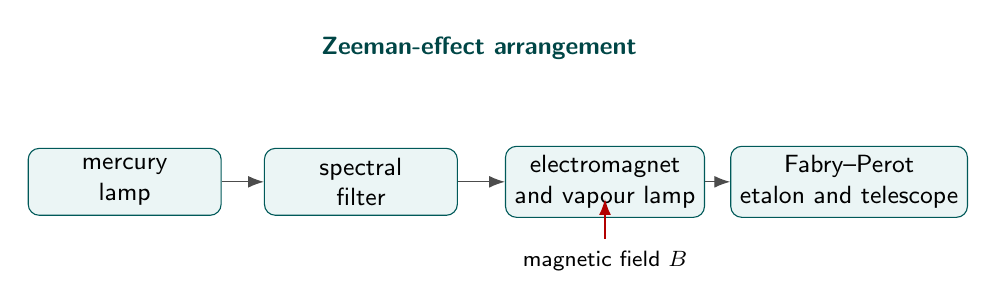
\begin{tikzpicture}[box/.style={draw=teal!70!black,fill=teal!8,rounded corners,minimum width=2.45cm,minimum height=.85cm,align=center,font=\sffamily\small},a/.style={-{Latex[length=2mm]},draw=black!70}]
\node[font=\sffamily\bfseries\small,text=teal!55!black] at (0,1.7) {Zeeman-effect arrangement};
\node[box] (lamp) at (-4.5,0) {mercury\\lamp};
\node[box] (filter) at (-1.5,0) {spectral\\filter};
\node[box] (magnet) at (1.6,0) {electromagnet\\and vapour lamp};
\node[box] (fp) at (4.7,0) {Fabry--Perot\\etalon and telescope};
\draw[a] (lamp)--(filter); \draw[a] (filter)--(magnet); \draw[a] (magnet)--(fp);
\node[font=\sffamily\footnotesize] at (1.6,-1.0) {magnetic field $B$};
\draw[-{Latex[length=2mm]},draw=red!70!black] (1.6,-.72)--(1.6,-.22);
\end{tikzpicture}
\end{document}
